
\documentclass[UTF8,a4paper]{ctexrep}
\usepackage{amsmath}
\usepackage{ctex}
\usepackage{titlesec}
\usepackage{multicol}
\usepackage{graphicx}
\usepackage{float}
\usepackage{wrapfig}
\usepackage{amsfonts,amssymb}
\usepackage[a4paper]{geometry}
\usepackage{CJK}
\usepackage{upgreek}
\usepackage{amsmath}
\usepackage{color}
\usepackage{titlesec}
\usepackage{mathtools}

\title{{\Huge 物理教程:从入门到入土}}
\author{{\large Alex Zhou}}
\date{{\large Start : 2023 年 4 月 21 日}}

\titleclass{\subsubsubsection}{straight}[\subsection]

\newcounter{subsubsubsection}[subsubsection]
\renewcommand\thesubsubsubsection{\thesubsubsection.\arabic{subsubsubsection}}
\renewcommand\theparagraph{\thesubsubsubsection.\arabic{paragraph}}

\titleformat{\subsubsubsection}
{\normalfont\normalsize\bfseries}{\thesubsubsubsection}{1em}{}
\titlespacing*{\subsubsubsection}
{0pt}{3.25ex plus 1ex minus .2ex}{1.5ex plus .2ex}

\makeatletter
\renewcommand\paragraph{\@startsection{paragraph}{5}{\z@}%
	{3.25ex \@plus1ex \@minus.2ex}%
	{-1em}%
	{\normalfont\normalsize\bfseries}}
\renewcommand\subparagraph{\@startsection{subparagraph}{6}{\parindent}%
	{3.25ex \@plus1ex \@minus .2ex}%
	{-1em}%
	{\normalfont\normalsize\bfseries}}
\def\toclevel@subsubsubsection{4}
\def\toclevel@paragraph{5}
\def\toclevel@paragraph{6}
\def\l@subsubsubsection{\@dottedtocline{4}{7em}{4em}}
\def\l@paragraph{\@dottedtocline{5}{10em}{5em}}
\def\l@subparagraph{\@dottedtocline{6}{14em}{6em}}
\makeatother

\setcounter{secnumdepth}{4} \geometry{left=2cm,right=2cm,top=2.8cm,bottom=3.2cm}
\setlength{\footskip}{3cm}
\setcounter{section}{-1}
\newcounter{defi}
\setcounter{defi}{0}
\newtheorem{de}[defi]{$\ \ \ \,\,\,$定义}
\newcounter{tdi}
\setcounter{tdi}{0}
\newtheorem{td}[tdi]{$\ \ \ \,\,\,$特点}
\newcounter{xzi}
\setcounter{xzi}{0}
\newtheorem{xz}[xzi]{$\ \ \ \,\,\,$性质}
\usepackage{hyperref} 
\begin{document}
	\maketitle 
	\setcounter{page}{0}
	%\usepackage[colorlinks,linkcolor=cyan]{hyperref}
	\section*{序:大道至简}
    欢迎来到《物理教程:从入门到入土》!首先请允许我代表本书全体编写成员对读者表示感谢.本书(由于厚度原因,其实更适合叫做讲义)追求大道至简的原则.世面上大部分物理相关的书籍都十分厚重,主要原因就是他们追求的是所谓严谨和完美.为了严谨性和实际性,它们花费大量笔墨于实验内容和"拓展阅读"(如"托里拆利发现大气压强的故事").我当然不是在贬低这些书.物理的源头当然是在一次次实验中产生的,但是我们不如把更多心思放在学系所必需的知识点上.譬如,数学计算.本书的设计理念便是如此:它旨在帮助大家复习和进一步拓展高中物理的主要概念,并同时致力于更多的数学问题求解.因此,无论是否第一次接触高中物理,还是为了备考竞赛,我认为那些太过无用的知识(如:匀速直线运动等内容)大可以进行省略.虽然我们删减了部分知识点,但书中每道例题都经过精挑细选并制定了详细的解答,既有简单的小试牛刀,更有综合性的过关斩将,难度分配均衡.同时,每一章节的习题部分虽然题目不多,但大多拥有极高的针对性.毕竟,在物理的学习中,我们更注重方法,而不是具体的计算,要明白题目的考点和解题步骤大纲,头脑中有很强的逻辑性,将千篇一律的解题步骤深深铭刻在脑海中.因此,我希望,也相信本书会对读者你有些帮助.此外,物理的学习不仅限于书面,我更希望你能将物理知识真正运用到实际问题中去.用一句话结束这个序吧:海阔凭鱼跃,天高任鸟飞.好运!(by编者小组·$\eta$)
	\section*{主编的话}
	欢迎同学们来到《物理教程:从入门到入土》.相信你在阅读此书之前,一定已经自己阅读了不少物理书籍吧.我认为,想要学好物理的关键不仅仅在于步步为营的精打细算,还有对每一个概念和知识点的清楚理解.我们先来讲讲书名吧.本来本书的名字定为《一本小物理书》.原因很简单,本书从厚度上来说并不算厚,因此还称不上是一本真正的、全面的物理书籍.而之所以改成了现在的《物理教程:从入门到入土》,主要是我们考虑到难度问题,从一开始的较为简易逐渐加难,直到高考压轴的相对论和我们补充的量子力学初步.请务必不要被它们的名称吓到!


	再来讲讲内容.每一个概念和知识点,我们深入浅出,以最直白的方式呈现出来.正如$\eta$所说的那样,我们追求所谓大道至简.再复杂的概念也能够以浅显的语言表述出来,哪怕是量子力学.阅读时,请务必\textbf{慢下来},放平心态.无论遇上什么样的困难都请不要放弃.我很欢迎读者们指出错误,也欢迎读者有关于物理的疑问向我提出.请电邮:ETRO\_gfyx@163.com. 


	最后,再来讲讲我为什么要写这本书.拥有一本属于自己的物理书(或者讲义)一直是我自幼以来的梦想,而如今有了这样做的能力,自然是第一时间写下来了.在我的物理学习过程中,使用的教材包括但不限于:《物理(实验班用)上册》\cite{25}《物理(实验班用)下册》\cite{26}《高中物理奥赛指导》\cite{27}.在我自己的学习过程中,它们略微有些不足以满足所有我的需求,因而希望这本书能帮到你.(by编者小组·$\omega$(主编))
	\newpage
	\section*{前言:学习指南}
	\paragraph{1.} \ \ \ \ 想必大家都看得出来,本讲义是由\LaTeX\cite{21}提供排版的.我非常喜欢这一排版工具,它比Word一类要好的多!\\以下文献可能可以帮助到你学习\LaTeX:\cite{22}\cite{23}\cite{24}
	\paragraph{2.} \ \ \ \ 本书中存在不少勘误,包括一些故意留下的,还有一些不小心留下的.那些故意留下的错误大多都标明了出来并希望读者给予修正,我希望通过这样增加作者与读者间的互动.
	\paragraph{3.} \ \ \ \ 讲义中不少公式是从Mathematica中引入,也有一些图片来自Python的matplotlib或Geogebra.它们是非常好的数学工具和图片引擎.强烈推荐它们!\\Mathematica官网直达:\href{https://www.wolfram.com/mathematica/}{\textbf{Mathematica}}\\Geogebra下载直达:\href{https://www.geogebra.org/}{\textbf{Geogebra}}\\本文电子版网页直达:\href{https://github.com/ZYpS-leader/Physics}{\textbf{电子物理书 }} 
	\paragraph{4.} \ \ \ \ 本书起稿于2023.4.21.
	\paragraph{5.} \ \ \ \ 一些常见问题的答案.\\\textbf{这本讲义(或者书)为什么这么薄?}这本书仅供学生自主学习(其实更多偏向复习),略去了一般教科书上的拓展内容等.我们去除了大部分的非专业性内容,但还是保留了一部分!\\\textbf{这本书上的推导过程有一些无法理解怎么办?}首先,本书中大量的使用了微积分技巧(如果你不清楚什么是微积分,建议阅读书目《普林斯顿·微积分读本》或你自己的高数教材).切记,在物理中数学往往是十分重要的!当然,不得不承认的是,为了减少篇幅,有一些过程出现了跳步.如果追求严谨,那你大可以去阅读《普林斯顿·数学分析读本》.那本书很适合你.此外,若仍然有对本书中表达式感到不解/奇怪,可能包括但不限于这些情况:\\1.没有积分主元.这种情况默认对时间$t$积分,也不排除对角度的积分.\\2.定积分无上下限.这种情况我们会在最后一步计算时加入,当然,这样写书是不好的!\\\textbf{如果我数学功底不好,还能继续阅读吗?}答案是肯定的.但还是那句话,数学在物理中相当重要.但在日常计算中,你可以使用如Mathematica等软件辅助.注意,这并非长久之计!\\\textbf{带**的章节是什么意思?}本书中有一些章节名字中带有**的标记.这意味着这一节是拓展阅读.不阅读它们不会对后续的学习造成影响,如果你不想学习得再深入些!
	\paragraph{6.}\ \ \ \  部分特殊字体演示:\\$\boldsymbol{\mathrm{F}}\to$向量(本例中为力F)的标量计算\\ $a\to$物理量(本例中为加速度a) \\\textbf{机械运动}$\to$特殊名词(本例中为机械运动)名称或例题/公式等的序号或超链接入口(包括类似\textbf{{\CJKfamily{zhkai} 这样的字体}})\\ {\CJKfamily{zhkai} 思考}$\to$一个需要你自己动手操作的例子(本例中为思考题)或某定理(或命题)的证明过程\\{\fangsong 补充}$\to$补充内容,即非必要阅读的内容\\\textsf{J}$\to$物理量的单位\\注:遇到$\pi$和$\uppi$,或\ .\ 和\ 。\ 一类意思相同但看起来不同的字母,不必惊慌,它们只是不同作者间未统一的格式... 
	\paragraph{7.最后,预祝同学们学习顺利!} 
	\begin{multicols}{2}
	\tableofcontents
	\end{multicols}{2}
	\newpage 
	\onecolumn
	\CTEXsetup[format+={\Huge}]{part}
	\CTEXsetup[format+={\huge}]{section} 
	\setcounter{page}{1}
	\part{ 经典物理学}
	 \chapter{运动学和力学}
 \section{运动学}
 运动学是物理四大基础学科之一,在各方面都起到了非常重要的奠基作用.因此,在第一章中,我们将一起探索运动的规律.
 \subsection{机械运动}
 首先,我们需要了解什么是\textcolor{red}{运动}.在物理中,运动可以分成\textcolor{red}{ 机械运动}和\textcolor{red}{非机械运动}.本章节中,主要以机械运动为核心展开.非机械运动,即波动,会在后续章节中讲到.
 \subsubsection{机械运动的定义和形式} 
 \subsubsubsection{机械运动的定义}
 \paragraph{机械运动} \ \ \ 从物理角度出发,包含了绝大多数宏观上的运动,但不包括大部分波动.机械运动需要选取合适的参考系(即惯性系)来分析问题.在\textcolor{red}{惯性系}中,惯性力也可以在受力分析时作为力出现,但此时的参考系不固定.我们会在第2章中详细讲到相关内容!
 \subsubsubsection{机械运动的形式}
 \paragraph{机械运动}\ \ \ 即一个物体相对于参考系中心(简单点说,另一个物体)产生了位移.通过计算加速度a、速度v、路程S等分析其运动状态,这就是本章的研究对象.常见的单物体机械运动包括:直线运动和曲线运动,又根据加速度不同分为匀速、匀加减速等.
 \subsection{匀速直线运动}
 此类运动问题更多的出现在数学中.由于它"匀速",因此$v_0=v_t$,且有$S=vt$,$a=0$两个结论.由于速度的不同和起始点的不同,出现了追及问题、相遇问题等,但它们一般较为简单(复杂的情况会在例题中进行讲解),这里不再展开.
 \subsection{匀加减速直线运动}
 在匀加减速直线运动中中,速度随时间的增加而增加,而单位时间的增加量叫做加速度a.速度和时间成线性变化,而路程是速度对时间的积分.通过以上定义不难得出有$S=\frac{1}{2}at^2+v_0t$和$v_t=v_0+at$.读者可以尝试自己证明一条引申公式:$\Delta S=\Delta(v^2)$或,$v^2_t-v^2_0=2as$.并不复杂!
 \subsection{平抛运动}
 抛体运动可将运动拆分成水平方向和竖直方向.
 在平抛运动中,水平方向分速度恒定,始终等于抛出时速度.与此同时在竖直方向上做自由落体运动,即加速度为g的匀加速运动.于是有$v_xt=v_0$,$v_yt=gt$,$S_xt=v_0t$,$S_yt=\frac{1}{2}gt^2$.思考:$\vec{S_t}$是多少?
 \subsection{斜抛运动}
 斜抛运动指以与地面有夹角$\theta$的初速度$v_0$抛出.不难发现竖直方向它的加速度仍然为g,但是先"上抛"再"下抛".先将初速度按方向分解,有$v_x=v_0\cos\theta$,$v_{y0}=v_0\sin\theta$.$v_x$保持不变,而$v_y$有向下的加速度g,即$v_{yt}=v_0\sin\theta-gt$.类似平抛运动,我们计算两个分方向的路程:$S_x=v_0t\cos\theta$,$S_y=v_0t\sin\theta-\frac{1}{2}gt^2$.不难看出,斜抛运动和平抛运动在水平分量上一致,即在水平方向分动能守恒.为什么呢?请先自己思考,我们将在第四章节中证明这个结论.
 \subsection{1.1例题}
 \paragraph{例1} 
 \ \ \ \ 两相同的小球从同一点以相同的初速度$v_0$斜向上抛出,A小球的初速度与水平地面夹角为$\alpha$,B小球的初速度与水平地面夹角为$\beta$.A小球经过时间$t_1$后落于地面上的C点.一定时间后B小球也落于C点.设起始点与C点的距离为$l$,则:\\(1)计算$l$;\\(2)$\alpha$和$\beta$的关系是?
 \paragraph{解}
 \ \ \ \ \  首先,设B小球运动时间为$t_2$,然后通过斜抛运动的公式有:$v_0\sin\alpha-t_1g=0,v_0\sin\beta-t_2g=0,v_0\cos\alpha t_1=l=v_0\cos\beta t_2$,那么第一问答案显而易见:$l=v_0\cos\alpha t_1$.然后联立两组等式,得$\sin\alpha=\frac{t_1g}{v_0},\sin\beta=\frac{t_2g}{v_0}$,即$\frac{\sin\alpha}{\sin\beta}=\frac{t_1}{t_2}$,同时$\frac{\cos\alpha}{\cos\beta}=\frac{t_2}{t_1}$,相乘得$\sin\alpha\cos\alpha=\sin\beta\cos\beta$,因此得解$\alpha=\beta$或$\alpha+\beta=0$或$\alpha=\pm(\pi/2\pm \beta)$.前两个解显然不合理,而$\alpha$和$\beta$都在开区间$(0,\pi/2)$中,因此最终得到答案$\alpha+\beta=\pi/2$.\\\ \ \ \ 这道题考验的是对斜抛运动两个公式的熟练运用,同时对数学公式有一定要求.本题中解的三角方程是典型的反三角方程,此类方程在物理中非常常用.同时还需要熟练掌握和差化积、积化和差、辅助角公式等.它们往往非常有用!
 \paragraph{例2} 
 \ \ \ \ 
 在水平平面上有两点点A、B.已知A点在B点左侧.小球$p_1$从B点以垂直于平面的速度$v_1$向上抛出.同时A点的小球$p_2$以与水平面夹角$\theta$的初速度$v_2$抛出(初速度向右).两球在时间t后相撞并停止运动.相撞点距离平面高度为h.求h的所有可能值和此时$\theta$需要满足的条件.
 \paragraph{解}
 \ \ \ \ 本题考察多解问题.有四种可能,分两类:$p_2$球速度向上时/向下时.每一类又分为两种可能:$p_1$球向上/向下.接下来我们分类讨论.\\
 \textbf{1:都在向上运动.}带入匀加速运动公式有$2gh=v^2_t=(gt)^2$,得到$h=\frac{1}{2}gt^2$.再带回$p_2$的斜抛公式,有$S_y=h=\frac{1}{2}gt^2=v_2t\sin\theta-\frac{1}{2}gt^2$,此时$\sin\theta=\frac{gt}{v_2},\theta=\arcsin\frac{gt}{v_2}$.\\
 \textbf{2.$p_1$向上,$p_2$向下.}从$p_1$的运动状态来看,仍然有$h=\frac{1}{2}gt^2$,但s$p_2$的状态略有改变.诶?好像还是$\theta=\arcsin\frac{gt}{v_2}$?对不对?有什么问题?尝试自己解答这个问题!\\
 \textbf{3.$p_1$向下,$p_2$向上.}$p_2$的高度还是$=v_2t\sin\theta-\frac{1}{2}gt^2$,但$p_1$的状态发生了改变.我们先计算$p_1$何时速度降低到0?很显然,$t_0=\frac{v_1}{g},S_1=\frac{v^2_1}{2g}$.此后再做匀加速运动时长$\frac{gt-v_1}{g}$,末态速度$gt-v_1$.路程$\Delta h=\frac{(gt-v_1)^2}{2g}$.然后带入$p_2$的斜抛,$v_2t\sin\theta-\frac{1}{2}gt^2=\frac{v^2_1-(gt-v_1)^2}{2g}=\frac{2v_1t-gt^2}{2}$.因此$\sin\theta=\frac{v_1}{v_2},\theta=\arcsin\frac{v_1}{v_2}$.\\
 \textbf{4.都在向下运动.}与第3种情况仅有略微的差异,不妨自己试试?\\\\
 {\CJKfamily{zhkai} 其实本题有些错误的地方,非常明显...试着把它们找出来并修正!}\\
{\CJKfamily{zhkai} 修正:}\_\_\_\_\_\_\_\_\_\_\_\_\_\_\_\_\_\_\_\_\_\_\_\_\_\_\_\_\_\_\_\_\_\_\_\_\_\_\_\_\_\_\_\_\_\_\_\_\_\_\_\_\_\_\_\_\_\_\_\_\_\_\_\_\_\_\_\_\_\_\_\_\_\_\_\_\_\_\_\_\_\_\_\_\_\_\_\_\_\_\_\_\_\_\_\_\_\_\_\_\_\_\_\_\_\_\_\_\_\_\_\_\_\_\_\_\_\_\_\_\\\_\_\_\_\_\_\_\_\_\_\_\_\_\_\_\_\_\_\_\_\_\_\_\_\_\_\_\_\_\_\_\_\_\_\_\_\_\_\_\_\_\_\_\_\_\_\_\_\_\_\_\_\_\_\_\_\_\_\_\_\_\_\_\_\_\_\_\_\_\_\_\_\_\_\_\_\_\_\_\_\_\_\_\_\_\_\_\_\_\_\_\_\_\_\_\_\_\_\_\_\_\_\_\_\_\_\_\_\_\_\_\_\_\_\_\_\_\_\_\_\_\_\_\_\_\_\_\\\_\_\_\_\_\_\_\_\_\_\_\_\_\_\_\_\_\_\_\_\_\_\_\_\_\_\_\_\_\_\_\_\_\_\_\_\_\_\_\_\_\_\_\_\_\_\_\_\_\_\_\_\_\_\_\_\_\_\_\_\_\_\_\_\_\_\_\_\_\_\_\_\_\_\_\_\_\_\_\_\_\_\_\_\_\_\_\_\_\_\_\_\_\_\_\_\_\_\_\_\_\_\_\_\_\_\_\_\_\_\_\_\_\_\_\_\_\_\_\_\_\_\_\_\_\_\_\\\_\_\_\_\_\_\_\_\_\_\_\_\_\_\_\_\_\_\_\_\_\_\_\_\_\_\_\_\_\_\_\_\_\_\_\_\_\_\_\_\_\_\_\_\_\_\_\_\_\_\_\_\_\_\_\_\_\_\_\_\_\_\_\_\_\_\_\_\_\_\_\_\_\_\_\_\_\_\_\_\_\_\_\_\_\_\_\_\_\_\_\_\_\_\_\_\_\_\_\_\_\_\_\_\_\_\_\_\_\_\_\_\_\_\_\_\_\_\_\_\_\_\_\_\_\_\_\\\_\_\_\_\_\_\_\_\_\_\_\_\_\_\_\_\_\_\_\_\_\_\_\_\_\_\_\_\_\_\_\_\_\_\_\_\_\_\_\_\_\_\_\_\_\_\_\_\_\_\_\_\_\_\_\_\_\_\_\_\_\_\_\_\_\_\_\_\_\_\_\_\_\_\_\_\_\_\_\_\_\_\_\_\_\_\_\_\_\_\_\_\_\_\_\_\_\_\_\_\_\_\_\_\_\_\_\_\_\_\_\_\_\_\_\_\_\_\_\_\_\_\_\_\_\_\_\\\_\_\_\_\_\_\_\_\_\_\_\_\_\_\_\_\_\_\_\_\_\_\_\_\_\_\_\_\_\_\_\_\_\_\_\_\_\_\_\_\_\_\_\_\_\_\_\_\_\_\_\_\_\_\_\_\_\_\_\_\_\_\_\_\_\_\_\_\_\_\_\_\_\_\_\_\_\_\_\_\_\_\_\_\_\_\_\_\_\_\_\_\_\_\_\_\_\_\_\_\_\_\_\_\_\_\_\_\_\_\_\_\_\_\_\_\_\_\_\_\_\_\_\_\_\_\_\\
 \subsection{1.1习题}
 \paragraph{}\ \ \ \ 本章的习题非常简单:证明1-6节中让你尝试证明的部分!
	\newpage
	 
\section{共点力平衡和力矩平衡} 
\subsection{共点力平衡}
虽然名字里带个平衡,但不代表本章的研究对象全部都受力平衡!本节旨在细致研究物体的受力情况,以便后续的学习.
\subsubsection{力的正交分解}
力$\boldsymbol{\mathrm{F}}$是一个矢量.这意味着它有方向!因此类似运动,我们可以将一个力分解在两个相互垂直的方向上.如图2-1所示.我们不妨设其中一个方向为x轴,另一方向为y轴,$\boldsymbol{\mathrm{F}}$与x轴的夹角为$\theta$,那么$F_x=F\cos\theta,F_y=F\sin\theta$,如图\ref{Fzjfj}所示.由此,我们将一个力$\boldsymbol{\mathrm{F}}$分解成了两个互相垂直的力.这就是力的正交分解.\begin{figure}[htp]\centering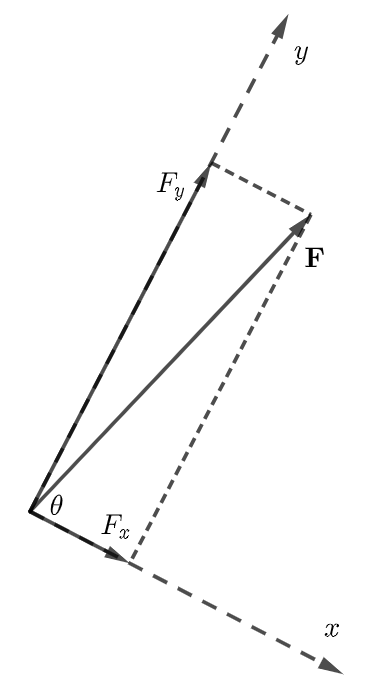
\includegraphics[width=3.5cm]{6-2}\caption[力的正交分解]{力的正交分解示意图}\label{Fzjfj} \end{figure}
\subsubsection{方向上的平衡}
在上一节中我们学会了如何将力$\boldsymbol{\mathrm{F}}$分解到两个方向.而所谓\textbf{平衡}想必大家都早有耳闻:这代表着在任何方向上(或某一特定方向上,如x轴或y轴)所受合理为零,表达式为:\begin{equation}
	\Sigma \boldsymbol{\mathrm{F}}_p=0
\end{equation}


其中$p$表示研究的某一方向.
\subsubsection{二力共线和三力共点}
接着延续上一节的结论:如果一物体所受合力为0,即$\Sigma  \boldsymbol{\mathrm{F}}_x=\Sigma \boldsymbol{\mathrm{F}}_y=0$,那么有: 
\newcounter{DL}[section]    %定义新计数器TH
\renewcommand{\theDL}{\thesection.\arabic{DL}}  %重新定义计数器命令\theTH的显示形式
\newcommand{\theorem}[1][]{\par\textbf{定理}\refstepcounter{DL}\textbf{\theDL}(#1)\quad}  %新定义定理命令
\theorem[平衡力]\label{dl1.1}


(1)如果该物体受两个力,那么它们共线等大;


(2)如果该物体受三个力,那么它们共点.

接下来我们证明\textbf{定理\ref{dl1.1}}.


{\CJKfamily{zhkai} 证明:}


{\CJKfamily{zhkai}\label{dl1.1-1} (1)如果该物体仅受恰好两个力,不妨设它们为$\boldsymbol{\mathrm{F}_1}$和$\boldsymbol{\mathrm{F}_2}$,并将$\boldsymbol{\mathrm{F}_1}$设为正方向,$\boldsymbol{\mathrm{F}_2}$与$\boldsymbol{\mathrm{F}_1}$的夹角为$\theta$.于是在$\boldsymbol{\mathrm{F}_1}$直线方向合力$F_1=\boldsymbol{\mathrm{F}_1}+\boldsymbol{\mathrm{F}_2}\cos\theta=0$,$F_2=\boldsymbol{\mathrm{F}_2}\sin\theta=0$,因此$\sin\theta=0$,所以$\theta=k\pi,k\in \mathbb{N}$.而如果$k\in \left\lbrace \mathbb{N}|k=2n,m\in N \right\rbrace $,此时$\boldsymbol{\mathrm{F}_1}+\boldsymbol{\mathrm{F}_2}=0$,又$\boldsymbol{\mathrm{F}_1},\boldsymbol{\mathrm{F}_2}>0$,矛盾.故$\theta=(2n+1)\pi,n\in\mathbb{N}.$这意味着$\boldsymbol{\mathrm{F}_1}$和$\boldsymbol{\mathrm{F}_2}$共线.且此时$\boldsymbol{\mathrm{F}_1}-\boldsymbol{\mathrm{F}_2}=0,$即$\boldsymbol{\mathrm{F}_1}=\boldsymbol{\mathrm{F}_2}$.}


{\CJKfamily{zhkai}\label{dl1.1-2-1} (2)如果该物体受三个力,还是设它们为$\boldsymbol{\mathrm{F}_1}$,$\boldsymbol{\mathrm{F}_2}$和$\boldsymbol{\mathrm{F}_3}$.仍然认为$\boldsymbol{\mathrm{F}_1}$为正方向,$\boldsymbol{\mathrm{F}_2}$与$\boldsymbol{\mathrm{F}_1}$夹角$\alpha$,$\boldsymbol{\mathrm{F}_3}$与$\boldsymbol{\mathrm{F}_1}$夹角$\beta$.类比\ref{dl1.1-1}的证明(1),有}\\
\[
\left\{  \begin{lgathered}
	\boldsymbol{\mathrm{F}_1}+\cos\alpha\boldsymbol{\mathrm{F}_2}+\cos\beta\boldsymbol{\mathrm{F}_2}=0\\
	\sin\alpha\boldsymbol{\mathrm{F}_2}+\sin\beta\boldsymbol{\mathrm{F}_3}=0
	\end{lgathered} \right.
\]


{\CJKfamily{zhkai} 这个方程其实并非最优证法.有兴趣的读者可以尝试解它.当然,一般来说,你会败兴而归.我们介绍一种更普遍、简单的办法:\\\textcircled{1} 将任意两个力分方向合成,使得$x$方向与$\boldsymbol{\mathrm{F}_1}$在同一直线.\\\textcircled{2}将合成所得的力与$\boldsymbol{\mathrm{F}_1}$再合成,利用\ref{dl1.1-1}的证明(1)的结论即可得到:两个力的合力和另一个力共线,这意味着它们一定共顶点!而两个力的合力一定经过它们的交点(如果有的话),因此这三个力共点.}\\


{\CJKfamily{zhkai} 思考:为什么两个力的合力一定经过它们的交点(如果有的话)?如果有四个力,}\textbf{定理\ref{dl1.1}}{\CJKfamily{zhkai} 还成立吗?需要做什么改动?}
\subsection{力矩平衡}
\subsubsection{力矩五要素和力矩的计算}
让我们回到正题.上一节中,我们讲了平衡力的一些性质.本节讲述力矩.


力矩$M$在初中已经学过,有五要素为支点O,动力(组)$F_1\sim F_n$,动力臂(组)$L_1\sim L_n$,阻力(组)$F_{n+1}\sim F_m$,阻力臂(组)$L_{n+1}\sim L_m$,其中$m>s$.每一个力$F_i$都有其对应的力臂$L_i$和力矩$M_i=F_iL_i$.


那力矩平衡的表达式?相信各位应该也不陌生吧:$\Sigma M_p=\Sigma M_q$.其中$M_p$和$M_q$分别表示动力力矩和阻力力矩.
\subsubsection{变力平衡}
当恒力或非恒力与物体以一夹角做功时,物体会改变运动状态.不同的角度和力都会对该力的力矩造成影响,而如果想不改变物体运动状态和力的方向(大小),我们就需要改变力的大小(方向).如果一个力作用在离支点O$l$的点A,力的方向与AO夹角为$\theta$,那么该力力矩为$M=Fl\sin\theta$,注意与运动学中更为常见的$\cos\theta$做区分.
\subsection{1.2例题}
\subsection{1.2习题}
	\newpage
	\section{牛顿三定律}
\subsection{牛顿第一定律:惯性}\label{gx}
\subsubsection{探究:惯性和什么有关?}
在初中物理中,我们已经学习了什么是\textbf{惯性}.那惯性有什么有关?有什么关?想必大家心中其实都有答案.本节就让我们再次走进惯性,看清其背后的本质!


先让我们回顾一下初中的惯性实验吧:我们将三个不同质量的小木块分别以相同初速度$v_0$滑上毛毯、木板和玻璃,比较它们停下来的位置.通过对比,我们发现:\textcircled{1}物体质量越大,停下来的越早;\textcircled{2}地面粗糙程度越大,物体停下来的越早.这意味着物体的\textbf{惯性}与它的质量和地面粗糙程度有关.所以\textbf{惯性}究竟是什么?揭晓答案:一个表述使物体运动状态发生改变难易程度的物理量.至于为什么和上述两个物理量有关,我们将在下一节中说明.
\subsection{牛顿第二定律:加速度和力的关系}
\subsubsection{$F=ma$}
从标题就知道,\textbf{牛顿第二定律}的表达式是$F=ma$.这意味着物体加速度与方向上受力成正比、与质量成反比.有眼尖的同学可能就要问了:等式左边的单位是牛(N),但右边却是千克·米/秒$^2$,这不是违背常理了吗?!我知道你很急,但你先别急,看看第\ref{lg}节吧!
\subsubsection{非惯性系}
在第\ref{gx}一节中,我们讲到了什么是惯性.但它并不是像力那样真实存在的东西,所以我们要引入一个\textbf{非惯性系}来描述它.别看标题以为这个系里没有惯性!它研究的正是惯性.在非惯性系中,将本来不可见的惯性具象化为一个力:$\boldsymbol{\mathrm{F}_v}$,它满足牛顿第二定律,只不过其中的速度$v$是相对于参考系中心的相对速度.因此,非惯性系在研究连接体问题等多物体运动时非常有用.
\subsubsection{再谈惯性}
在\ref{gx}一节中,我们留下来一个问题:\emph{为什么惯性和物体在方向上的速度无关,但和粗糙程度和质量有关?}在学过牛顿第二定律后,相信你能自己解决这个问题.事实上,由于在水平方向上物体的运动只受摩擦力$f$影响,因此$f$的大小决定了它的惯性.由公式可知,$f=\mu N=ma$,因此$a=\frac{\mu N}{m}=\mu g$,因此惯性和物体质量、粗糙程度有关.

\subsection{牛顿第三定律:作用力与反作用力}
\subsubsection{证明:作用力与反作用力矢量和为0}
牛顿第三定律告诉我们,如果两个物体有接触并相互作用,保持平衡(即一起做匀速直线运动或同时静止),那么它们间的作用力等于对方的反作用力.很好证明:在\textbf{定理\ref{dl1.1}}中,我们知道它们间的一对反作用力共线;而他们保持平衡,因此合力为0.
\subsection{**量纲**}\label{lg}
\subsubsection{什么是量纲}
我们知道,在国际单位制中,有这7个基本单位:\footnote{本节中标点符号不同于前文,它们是中文(全角)标点,但意思没有任何区别.不过是不同作者的习惯不同!——审核注}
\begin{equation*}
    \mathrm{m}\qquad\mathrm{kg}\qquad\mathrm{K}\qquad\mathrm{s}\qquad\mathrm{cd}\qquad\mathrm{mol}\qquad\mathrm{A}
\end{equation*}

它们分别代表长度、质量、温度、时间、光强、物质的量、电流的单位。而生活中或学术中的各种单位,都可以由这七个基本单位通过乘法、除法、乘幂的组合导出,它们就是导出单位\footnote{平面角度和立体角度例外,你可以将它视为无单位数——作者注},如$\mathrm{J}$、$\mathrm{V}$、$\mathrm{Pa}$等。为了表明物理量之间的关系,人们引入了\textbf{量纲}这一概念。

长度、质量、温度、时间、光强、物质的量、电流的量纲分别表示为\(L\  M\  \Theta\  T\  J\  n\  I\);而一个物理量$X$的量纲用\(\dim X\)来表示,简写为$[X]$。比如
\[
    \dim v = LT^{-1}\qquad \qquad \dim W = ML^2T^{-2}
\]

\subsubsection{量纲的应用}
\emph{量纲有什么作用呢?}

想象一个场景:你在一次物理考试中,有一道题需要用到开普勒第三定律
\[
    T = 2\uppi \sqrt{\frac{R^3}{\mathrm{G}M}}
\]
但你死活背不出来。你只记得系数是$2\uppi$。在这种情况下,你就可以运用到量纲分析法了。发挥你的头脑风暴,思考:天体的运动周期和哪些量有关呢?首先,天体受到引力的吸引,因此和万有引力常数\(\mathrm{G}\)有关,还和母星质量有关(这里我们假设行星质量$\ll$母星质量)。再根据开普勒第三定律的文字表述(不会有人连这个都背不下来吧)得到这和行星到母星的距离(这里假设行星质量忽略不计,也没有初速度,所以行星以匀速圆轨道运行)有关。综上,我们不妨设
\[
    T = 2\uppi R^\alpha G^\beta M^\gamma
\]
由于\(\dim\mathrm{G} = L^3M^{-1}S^{-2}\qquad\dim R = L\qquad\dim M = M\qquad\dim T=T\),故
\[
    \left\{\begin{lgathered}
        3\beta+\alpha=0\\
        -\beta+\gamma=0\\
        -2\beta=1
    \end{lgathered}\right.
\]
可解出未知数,再代入原式中,公式也就出来了。
\subsection{1.3例题}
\subsection{1.3习题}
	\newpage
	\section{能量学定律}
在前几节中,我们讲了\textbf{运动学}、\textbf{牛顿三定律}和\textbf{力的合成与分解}.它们是经典物理学的重要组成部分,而为了进一步加强它们间的联系,我们进一步引入\textbf{能量}的概念.
\subsection{能量守恒定律}
什么是\textbf{能量}?所谓\textbf{能量}其实就是一个物体(或系统)所能做功的本领,用$E$表示,国际单位J,且$\dim J=kg\cdot m^2/s^2$.($\dim$是什么意思?参见\textbf{\ref{lg}一节.})此外还有单位如电子伏特ev等单位.电子伏特\textsf{ev}将在\textbf{\ref{dsn}}中提到.


回到能量守恒定律.我们已经了解了什么是\textbf{能量},那\textbf{能量}的大小和公式是什么?它就是大家耳熟能详的质能方程$E=mc^2$.\textbf{注意!它仅建立在狭义相对论上!}那它满足什么条件呢?


在大自然中所有物体的能力总和均保持不变.在任何情况下\textbf{都}保持不变!也可以仅考虑一个系统中的能量之和守恒,但此时该系统必须\textbf{孤立}外部,避免能量增加或损失.
\subsection{动能定理}\label{dndl}
还是先来回顾下什么是\textbf{动能}.动能$E_k=\frac12mv^2$,文字表达为一物体的动能与该物体质量和速度的平方成正比.看到刚刚讲过的\textbf{能量守恒定律},该物体哪怕不孤立于外界,但是它所损失的势能即为它增加的动能,表达式为$\Delta E_k=\Sigma W$,即动能变化量等于合外力做功.该等式在任何条件下成立,无需前提. 
\subsection{机械能守恒}
什么是\textbf{机械能}?机械能为动能$E_k$和势能$E_p$(仅包括重力势能和弹性势能).在\textbf{\ref{dndl}}中,我们知道动能的变化量是合外力做功,而势能的改变必有外力做功.与此同时,外力$F$做功意味着物体将有速度$v$的变化.这两个力必定相反.于是当且仅当动能 的变化量刚好等于势能变化量的相反数时,机械能守恒.而此时受到两个外力的矢量和为0,故合外力为0.


因此机械能守恒公式表达为$ E=E^{'}$  ,iff $F_{\mbox{\scriptsize 合}} =0$. 
\subsection{动量和冲量定律}
\subsubsection{动量和冲量}
什么是\textbf{动量}?动量是描述一个物体运动能力的物理量,用符号$p$表示,对任意物体有$p=mv$,其中$v$为物体当前的运动速度.


什么是\textbf{冲量}?冲量是描述一个力所做功多少的量,注意与功$W$区分.冲量用符号$I$表示,对力有$I=Ft$,$t$为该力做功时间.
\subsubsection{动量守恒}
当一个物体所受合外力为0时,它的运动状态不会发生改变,即速度$v=v^{'}$.如果该物体质量守恒,那么显然有$p=p^{'},mv_1=mv_2$.如果它质量改变呢?那根据牛顿第二定律显然加速度减小,速度减小.如果只是单纯的改变质量,那速度应当恰好和质量成反比,仍然有$p=p^{'},mv_1=mv_2$.
\subsubsection{动量定律}
要改变物体的动量$p$,就需要一个外力来改变它的速度.我们会自然的想到冲量$I$.那$p$和$I$之间有什么关系呢?


我们不妨做一下计算.先假设物体质量不变,那么有 
\begin{align}
&\Delta p_{1\to 2}(\mbox{即1状态到2状态的动量变化量})\notag 
\\={}& m_1v_1-m_2v_2(\mbox{拆分两个动量})\notag 
\\={}&m\Delta v(\mbox{由于质量相等,提取公因式m})\notag 
\\={}&m(a\Delta t_{1\to 2})(\mbox{由运动学公式$\Delta v=a\Delta t$})\notag 
\\={}&(ma)t(\mbox{重新组合三个量})\notag 
\\={}&Ft=I(\mbox{由牛二有$F=ma$})
\end{align}
因此有$\Delta p=I$.
\subsection{**其他能量**}
在此节中简要介绍一下能量$E$的单位.
\paragraph{1.J}\qquad 这是能量的国际单位,$1 \textsf{J}=$\textsf{$kg\cdot m^2/s^2$}.
\paragraph{2.ev}\qquad 电子伏特,表示一个单位元电荷(带电量为$1.6\times 10^{-19}\textsf{C}$)通过一个单位电场(电压为1V的电场)所获得的的动能,$1\ \textsf{ev}=1.6\times 10^{-19}\textsf{J}$.
\paragraph{3.cal}\qquad 卡路里,表示1克水(标准水,即密度恰好为$1\times 10^3kg/m^3$)在一个标准大气压下升高一度所需要的热量.$1\ \textsf{cal} =4.19J $.

\paragraph{4.erg}\qquad 尔格.这个单位非常非常少用,在此仅做补充.一尔格的能量能使一达因的力让物体在力的方向上移动1厘米.一达因的力可以使一个质量是1克的物体产生$1\times 10^{-2}m/s^2$的加速度.
\subsection{1.4例题}
\subsection{1.4习题}
	\newpage
	\section{圆周运动和简谐振动}
\subsection{圆周运动}
\subsubsection{向心力和向心加速度}
\subsubsection{角速度、角动量和曲率半径}
\subsubsection{变速圆周运动}
\subsection{简谐振动}
\subsubsection{波、波长和频率}
\subsubsection{回复力}
\subsubsection{两种波动图像的阅读}
\subsubsection{特殊的简谐振动:单摆}
\subsection{1.5例题}
\subsection{1.5习题}
	\newpage
	\section{宏观力学和运动学综合}
\subsection{综合例题1}
\paragraph{例1}\ \ \ \ 一弧形轨道AB如图6-1,最高点A的高度为$h$.其上任意一点C,满足该点高度$h_C=h_1,\rho_C=h^2_1+\rho_0$,其中$\rho_C$为C点曲率半径,$\rho_0$为轨道最低点B点曲率半径.一质量为$m$的小球从A点静止释放,问当小球与轨道间的摩擦系数$\mu$取何值时,小球下落到B点再次静止?\\\begin{wrapfigure}{r}{3.5cm}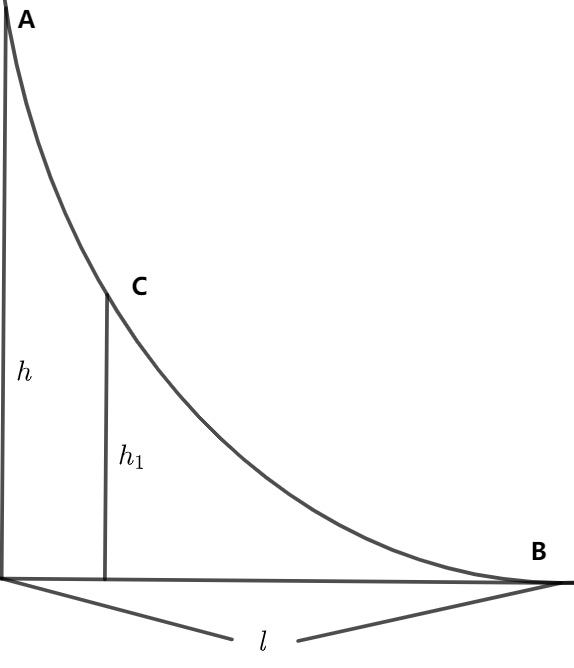
\includegraphics[width=3.5cm]{6-1}\end{wrapfigure}
	
\subsection{综合习题1}
	\newpage
	\chapter{光和声}
\section{光}
\subsection{波动光学}
\subsubsection{光波}
\subsubsection{光的更多性质}
\subsection{再谈光的折射} 
\subsubsection{折射率}
\subsubsection{光的衍射现象}
\subsection{光的粒子性和波动性}
\subsubsection{波动性}
\subsubsection{粒子性}
\subsection{2.1例题}
\subsection{2.1习题}
	\newpage
	\section{声}
\subsection{多普勒效应}
\subsubsection{多普勒效应的公式和证明} 
\subsection{2.2例题}
\subsection{2.2习题} 
	\newpage
	\part{前现代和近现代物理学}
	\chapter{电与电磁} 
\section{静电场}
\subsection{静电}
\subsection{电流}
\subsubsection{电流}
\subsubsection{电压和电阻}
\subsubsection{再谈欧姆定律}
\subsubsection{电流成因}
\subsection{电子}
\subsubsection{**化学向物理(1)**}
\subsubsection{电荷}
\paragraph{库仑定律}\ \ \ \ 
\subsection{3.1例题}
\subsection{3.1习题}
	\newpage
	\section{再谈电学:电场、电势和电容}
\subsection{点电荷}
点电荷是一个带电质点,是宏观层面的,注意与第9章中的微观电子区分.
\subsection{电场和场强}
\paragraph{电场:}\ \ \ \ 电场是电荷及变化磁场周围空间里存在的一种特殊物质.不可见但真实存在.其强度记为$E$.场强为矢量,方向与正电荷在电场中受力方向相同.
\paragraph{电场力:}\ \ \ \ 电场力$\boldsymbol{\mathrm{F}}$ 是由电场而产生的力,是宏观力,满足牛二$F=ma$.
\subsubsection{定义式和决定式}
\paragraph{场强定义式:}\ \ \ \ 电荷受到电场力F和其带电量q的比值定义为所在电场场强:\begin{equation}\vec{E}=\frac{\vec{F}}{q},E=\frac{F}{q} \end{equation}\paragraph{场强决定式:}\ \ \ \ 一检验电荷所受场强与产生电场的点电荷带电量成正比,与两电荷距离平方成反比:\\\begin{equation}\label{cqjds} E=\frac{kQ}{r^2}\end{equation}\paragraph{注意!}\ \ \ \  在\textbf{公式\ref{cqjds}}中,当$r\to0$时,不能视为$E\to\infty$!
\subsubsection{电场叠加原理}
任一点所受场强等于所有方向的电场场强之和.\[E_{\mbox{\scriptsize 合}}=\sum E\] 
 

\subsection{电势和电势能}
\subsubsection{电势}
什么是\textbf{电势}?为了描述一个电荷在电场内所受电场力做功的大小,引入了电势$\varphi$.两点间的电势差$U=\Delta\varphi$.
\subsubsection{电势能}\label{dsn}
什么是\textbf{电势能}?为了描述一个电荷在电场内所受电场力做功的能力,引入了电势能$E_p$,满足对于一点电荷有$E_p=q\varphi$.电势能的减小意味着电场力做功.由电势能反推可得电势,电势为标量且有正负.电势一般表示相对电势,在大部分情况下,记一定点或无穷远处电势为零从而计算相对电势. 


对于电场力做功,有\[W_{\mbox{\scriptsize 电}}=\Delta E_{p\mbox{\scriptsize 减}}=q\Delta\varphi=qU\]
\subsubsection{静电场的环路定理}
在一个电场中,一个电荷绕某一电环一圈,电势降落为零,表达式为\[\oint\vec{E}\mathrm{~d}\vec{l}=\oint\mathrm{~d}U=\oint q\vec{E}\mathrm{~d}\vec{l}=0\]
\subsection{电场线和等势线}
\subsubsection{电场线}
\textbf{电场线}是引入的假想曲线,用来表现电场的方向和大小.任意一个电场都有对应的电场线.用电场线的疏密表示该处的电场大小. 电势由电场线方向降落,电场线方向是唯一电势降落最快的方向.电场中的电场力方向就是电场线方向.
\subsubsection{等势线}
\textbf{等势线(面)}由一系列电势相等的点构成,因此\textbf{等势线(面)}上所有点的电势相等.一簇等势线(面)中相邻两个等势线(面)之间的电势差$U$相等.
\subsubsection{电场线和等势线的性质}
\paragraph{性质1}\qquad 电场线和等势线处处垂直;
\paragraph{性质2}\qquad 电场线由电势高的等势线指向电势低的等势线;
\paragraph{性质3}\qquad 任意两等势线(面)不相交、不相切;
\paragraph{性质4}\qquad 在等势线(面)上移动电荷,电场力不做功,电势能不变;
\paragraph{性质5}\qquad 等势线(面)的疏密表示了电场强度的大小,法线方向表示场强方向.\\\\
{\CJKfamily{zhkai} 思考:为什么等势线两两不相交、相切?(提示:从场强出发)}
\subsection{静电平衡}
\subsubsection{静电平衡的状态特点}
\begin{td}\qquad 平衡的导体内部场强处处为零且误电场线;\end{td}
\begin{td}\qquad 导体表面上任一点的电场线方向与表面垂直;\end{td}
\begin{td}\qquad 导体表面附近的场强$E=4k\uppi\sigma$($\sigma$为导体表面电荷面密度);\end{td}
\begin{td}\qquad 导体表面的场强$E=2k\uppi\sigma$($\sigma$为导体表面电荷面密度);  \end{td}
\paragraph{}\qquad {\CJKfamily{zhkai} 思考:为什么导体表面附近的场强恰好等于其表面场强的两倍?(提示:从电场叠加原理出发)}
\begin{td}\qquad 均匀带电$Q$,半径为$R$的小球外侧附近场强为$\frac{kQ}{R^2}$,表面场强为$\frac{kQ}{2R^2}$;\end{td}
\begin{td}\qquad 整个导体是等势体,导体表面是等势面;\end{td}
\begin{td}\qquad 净电荷只分布在导体表面上,导体内部无净电荷;\end{td}
\begin{td}\qquad 空腔导体因为内部空腔且无电场,所以可以屏蔽外部电场,即\textbf{静电屏蔽}.\end{td}
\subsubsection{静电平衡的前因后果}
\paragraph{1.静电间的相互作用}\qquad 电荷同性相斥异性相吸 
\paragraph{2.静电感应}\qquad 正电荷沿电场线方向移动,负电荷沿电场线反方向移动 
\paragraph{3.静电平衡}\qquad 8个性质 
\paragraph{4.静电屏蔽效应}\qquad
\subsection{电容}
\subsubsection{电容器}
\begin{de}两个相互靠近但\textbf{相互绝缘}的导体构成一个\textbf{电容器}.\end{de}
\subsubsection{电容}
\begin{de}电容器所带电量与两极板电势差的比值定义为\textbf{电容}.\end{de}


因此有定义式\begin{equation}
	C=\frac{Q}{U}
\end{equation}
电容由两极板形状、大小、正对面积、相对位置、材料、电介质的介电常数等决定,与$Q$和$U$无关.材料电容反应其容纳电荷的本领大小,单位\textsf{F},$1\textsf{F}=1\frac{c}{V}, 1\textsf{F}=1\times10^6\mu F=1\times10^{12}pF.$
\subsubsection{特殊电容器}
\subsubsubsection{平行板电容器}
两个\textbf{等大的}正对的相距较近\footnote{此处较近指远小于无穷大——编者注}的彼此绝缘的平行金属板称为\textbf{平行板电容器}.
\paragraph{平行板电容器的电容}\ \\


\qquad$C=\frac{Q}{U}$\qquad$U=Ed$\qquad$E=4\pi k\sigma$\qquad$\sigma=\frac{Q}{S}$


其中$Q$为带电量,$U$为两板间电势差(即电压),$E$为两板间场强,$d$为两板间距离,$\sigma$为电荷面密度,$S$为两板正对面积.


综合四个基本公式,有$C=\frac{S}{4\pi kd}$.
\subsubsubsection{孤立导体球}
\paragraph{孤立导体球的电容}\ \\
\qquad$C=\frac{Q}{U}$\qquad$U=\frac{kQ}{r}$


其中$Q$为带电量,$U$为电压,$r$为球体半径.
\subsubsection{电容器的储能}
\begin{td}
与电源保持连接时,电压不变.
\end{td}\begin{td}充电后断开电源,电量不变.\end{td}
\subsection{带电粒子在匀强电场中的运动}
\subsubsection{加速运动}
一般使用动能定理:$qU=\frac12m{v_t}^2-\frac12m{v_0}^2$.一般的加速电场如图\ref{jsdc}所示.\begin{figure}[htp]\centering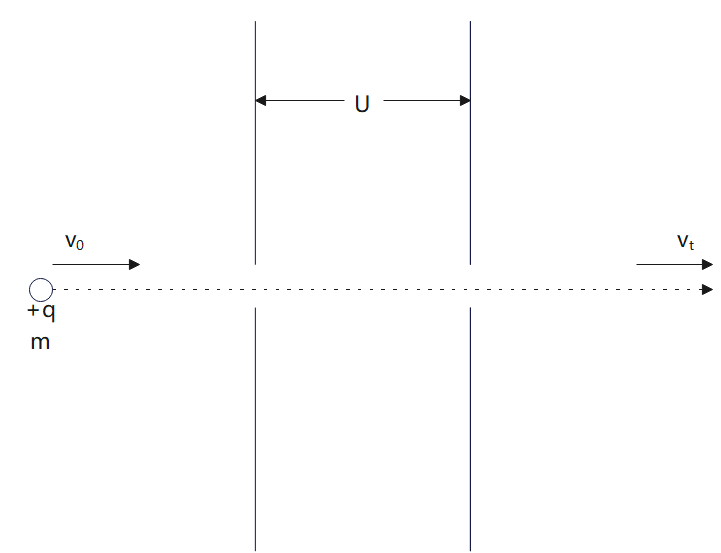
\includegraphics[width=8cm]{11-1}\caption[加速电场示意图]{加速电场示意图}\label{jsdc} \end{figure}
\subsubsection{偏转运动}
受不同电场叠加影响而发生场内偏转时,速度也会随之受到影响.如图\ref{pzdc}\begin{figure}[htp]\centering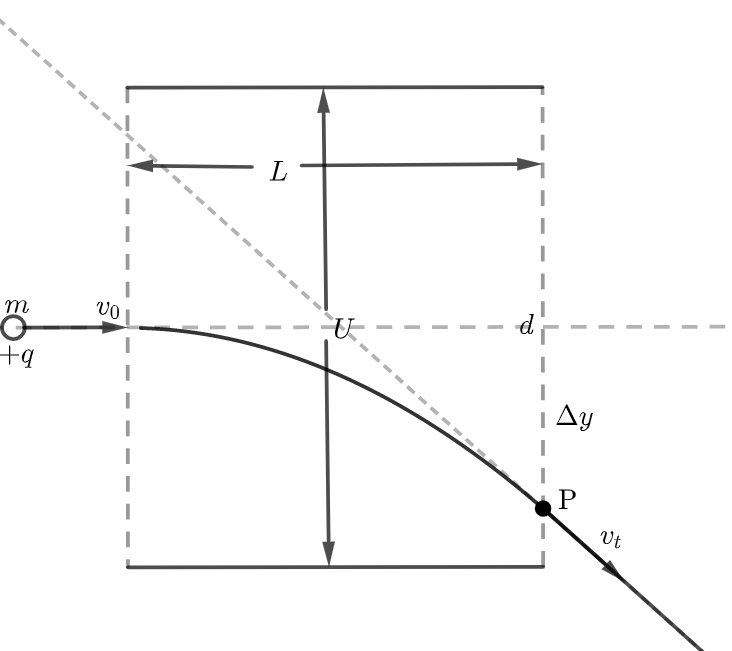
\includegraphics[width=4cm]{11-2}\caption[偏转电场示意图]{偏转电场示意图}\label{pzdc} \end{figure}\newpage


让我们仔细分析一下该偏转电场.两均匀带电板间间隔为$d$,电势差为$U$,长度均为$L$,一质量为$m$、带$+q$的小球以初速度$v_0$沿两板中线进入由两板构成的电容器中(不计重力)且飞出时未触碰到下板,求飞出点P距离中线距离和末速度$v_t$.
\begin{de}射出点与射入点连线与中线夹角$\theta$称为\textbf{电场偏转角};[射出点/与/(射出时速度反向延长线)与(中线)交点/连线]/与中线夹角$\alpha$/称为\textbf{速度偏转角}.\footnote{本句较长且均为\ 与\ 字,因此用/和括号来分割句子以便理解.}\end{de}


在场中的运动是类平抛运动.加速度\begin{equation*}a=\dfrac{qU}{md}\end{equation*} 时间\begin{equation*}
	t=\dfrac{L}{v_0}
\end{equation*}
 故竖直($y$方向)位移\begin{equation*}y=\dfrac{1}{2}\dfrac{qU}{md}({\dfrac{L}{v_0}})^2=\dfrac{qUL^2}{4E_{k}d}\end{equation*}
有\begin{equation*}
	\tan\alpha=\dfrac{v_y}{v_0}=\dfrac{qUL^2}{4E_kdv_0}=\dfrac{qUL^2}{2m{v_0}^3d} 
\end{equation*}
$\tan\theta$的推导十分类似,请读者自己完成推导.
[注意!]$\tan\theta$的结果应为\begin{equation*}\tan\theta=\dfrac{qUL^2}{4mv_0^3d}=\dfrac{1}{2}\tan\alpha\end{equation*}
\subsection{3.2例题}
\paragraph{例1}\qquad a
\subsection{3.2习题}
	\newpage
	\section{磁}
\subsection{电与磁的关系} 
\subsection{磁场和场强}
\subsubsection{定义式和决定式}
\subsection{磁感线}
\subsection{通电螺线管}
\subsection{磁通量}
\subsection{电磁感应}
\subsection{3.3例题}
\subsection{3.3习题}
	\newpage
	\section{电磁学和热力学综合}
\subsection{综合例题2}
\subsection{综合习题2} 
	\newpage
	\chapter{热力学和流体力学}
\section{分子动理论}
\subsection{分子模型}
\subsubsection{分子}
\subsubsection{分子力和范德华力}
\subsection{热力学}
\subsubsection{分子间的动能}
\subsubsection{热能}
\subsubsection{热膨胀和热传递}
\subsubsection{三条热能公式}
 
\section{气体实验}
\subsection{三大气体实验定律}
\subsection{理想气体方程}
\subsection{气体压强}

\section{流体力学}
\subsection{液体表面张力}
\subsection{液体的浸润}
\subsection{液体中物体所受阻力的探究}
\subsection{伯努利原理}
\subsection{液体压强和大气压强} 
\subsection{第4章例题}
\subsection{第4章习题}

	\newpage 
	\part{近代物理和天体物理学初步}
	\chapter{天体物理学初步}
\section{宏观宇宙}
\subsection{太阳系和银河系}
\subsection{天体间的万有引力}
\subsection{潮汐力和洛希极限}
\subsection{自转和公转的成因}
\subsection{天体运动轨道的计算}
\subsection{外天体探索}
\section{微观宇宙}
\subsection{宇宙起源}
\subsection{夸克和中微子}
\subsection{**化学向物理(2)**}
\section{第5章例题}
\section{第5章习题}
	\newpage
	\chapter{近代物理学初步}
\CTEXsetup[format+={\Large}]{section} 
\section{近代物理那些事}
\subsection{近代物理的发展史}
\paragraph{近代物理是从什么时候开始的?}\ 
\\1897年的Thomson发现电子以来,自此拉开了近代物理学的序幕.包括此前伦琴所发现的\textbf{X射线}和贝克勒尔发现的\textbf{物质放射性},以及之后普朗克、爱因斯坦、薛定谔、波尔、泡利和古兹密特等人的成果并称为旧量子学.
\paragraph{从微观到宏观,究竟是什么样的进步?}\ 
\\从以牛顿力学为基础的经典力学出发,我们有了宏观物理学,也就是所谓\textbf{经典物理学}.而自近代以来,科学的飞速进步让人们有了进入微观世界能力.从此我们可以更深入的观察微观粒子间的关系,去探究神秘的微观世界.那就让我们带着对以上各位近代物理学家的敬仰,一同走进近代物理学的世界! 
\subsection{什么是近代物理}
\textbf{近代物理}\cite{28}主要研究的是量子力学和相对论
\section{微观模型:让我们再深入些}
\section{量子力学初步}
\subsection{什么是量子力学}
\subsection{泡利不相容}
\subsection{物质波}
\subsection{波粒二象性}
\subsection{量子纠缠}
\section{第6章例题}
\section{第6章习题}
	\newpage
	\part{综合复习}
	\CTEXsetup[format+={\huge}]{section} 
	\chapter{综合复习}
\section{综合例题3}
\newpage
\section{综合习题3-1}
\newpage
\section{综合习题3-2}
	\newpage
	\part{后记}
	\section*{致谢} 
	感谢阅读致谢.
	
	
	首先请允许我作为本书主编感谢所有直接或间接参与了本书编写的人员.他们包括:我的数学和物理老师、同学和ETRO学习小组的成员们.
	
	
	感谢CSDN、Git和\TeX 社区的人们,他们提供了大量可靠的排版方式,才有了这样的一本书.当然也归功于这两个网站的工作人员!(本文电子版便发布在\href{https://github.com/ZYpS-leader/Physics}{\textbf{Github}}以完全开源使用)
	
	
	感谢每一位在我物理学习和信息技术中提供过帮助的人们,包括一些完全陌生的人们.
	
	
	感谢每一位我曾经遇到过的优秀的人们:感谢你们激励我学习,并写下这本书.
	
	
	致每一位对物理热爱的你:愿物理成为生命中的那道光.
	\addcontentsline{toc}{section}{致谢}
	\newpage
	 
	\bibliographystyle{unsrt}
	\bibliography{cxk.bib}	
	\addcontentsline{toc}{part}{参考文献}	 
	 
	
\end{document}